%% %%%%%%%%%%%%%%%%%%%%%%%%%%%%%%%%%%%%%%%%%%%%%%%%%
%% Work of Baeza Olvera Daniel Jesus, making use of this template, all credits due to the original creaters below:
%% Template for a conference paper, prepared for the
%% Food and Resource Economics Department - IFAS
%% UNIVERSITY OF FLORIDA
%% %%%%%%%%%%%%%%%%%%%%%%%%%%%%%%%%%%%%%%%%%%%%%%%%%
%% Version 1.0 // November 2019
%% %%%%%%%%%%%%%%%%%%%%%%%%%%%%%%%%%%%%%%%%%%%%%%%%%
%% Ariel Soto-Caro
%%  - asotocaro@ufl.edu
%%  - arielsotocaro@gmail.com
%% %%%%%%%%%%%%%%%%%%%%%%%%%%%%%%%%%%%%%%%%%%%%%%%%%
\documentclass[11pt]{article}
\usepackage{UF_FRED_paper_style}
\usepackage{lipsum}  %% Package to create dummy text (comment or erase before start)

%% ===============================================
%% Setting the line spacing (3 options: only pick one)
% \doublespacing
% \singlespacing
\onehalfspacing
%% ===============================================

\setlength{\droptitle}{-5em} %% Don't touch

% %%%%%%%%%%%%%%%%%%%%%%%%%%%%%%%%%%%%%%%%%%%%%%%%%%%%%%%%%%
% SET THE TITLE
% %%%%%%%%%%%%%%%%%%%%%%%%%%%%%%%%%%%%%%%%%%%%%%%%%%%%%%%%%%

% TITLE:
\title{Applied Data Science Capstone: The Battle of Neighborhoods
\thanks{Presentation for the Capstone project, part of Applied Data Science Specialization, Coursera.}
}

% AUTHORS:
\author{Baeza Olvera Daniel Jesus\\% Name author
    \href{mailto:dbaeza@ibm.com}{\texttt{dbaeza@ibm.com}} %% Email author 1 
%\and Forth Author\\% Name author
%    \href{mailto:forthuthor@ufl.edu}{\texttt{forthuthor@ufl.edu}}%% Email author 4
    }
    
% DATE:
\date{\today}

% %%%%%%%%%%%%%%%%%%%%%%%%%%%%%%%%%%%%%%%%%%%%%%%%%%%%%%%%%%
% %%%%%%%%%%%%%%%%%%%%%%%%%%%%%%%%%%%%%%%%%%%%%%%%%%%%%%%%%%
\begin{document}
% %%%%%%%%%%%%%%%%%%%%%%%%%%%%%%%%%%%%%%%%%%%%%%%%%%%%%%%%%%
% %%%%%%%%%%%%%%%%%%%%%%%%%%%%%%%%%%%%%%%%%%%%%%%%%%%%%%%%%%
% ABSTRACT
% %%%%%%%%%%%%%%%%%%%%%%%%%%%%%%%%%%%%%%%%%%%%%%%%%%%%%%%%%%
% %%%%%%%%%%%%%%%%%%%%%%%%%%%%%%%%%%%%%%%%%%%%%%%%%%%%%%%%%%
{\setstretch{.8}
\maketitle
% %%%%%%%%%%%%%%%%%%
\begin{abstract}
% CONTENT OF ABS HERE--------------------------------------
As part of the IBM \& Coursera Applied Data Science Specialization, it is required to do a small research using the taught data science methodologies and data sources.
The data science methodologies and data sources that had more emphasis were, Geographical Data with the Python package Folium, and the usage of third party APIs for retrieval of location data.
\newline

The problem that this little research tackles is about Food Venues, especially Mexican Food venues in the city of Naha, Okinawa Japan which is the place I wish to live in the not so distant future. One of my plans while living there is Co-owning a Mexican Food restaurant.
% END CONTENT ABS------------------------------------------
\newline

\noindent
\textit{\textbf{Keywords: }%
Data Science; Foursquare; GIS; Google Maps API; Capstone, Python.} \\ %% <-- Keywords HERE!
\end{abstract}
}

% %%%%%%%%%%%%%%%%%%%%%%%%%%%%%%%%%%%%%%%%%%%%%%%%%%%%%%%%%%
% %%%%%%%%%%%%%%%%%%%%%%%%%%%%%%%%%%%%%%%%%%%%%%%%%%%%%%%%%%
% BODY OF THE DOCUMENT
% %%%%%%%%%%%%%%%%%%%%%%%%%%%%%%%%%%%%%%%%%%%%%%%%%%%%%%%%%%
% %%%%%%%%%%%%%%%%%%%%%%%%%%%%%%%%%%%%%%%%%%%%%%%%%%%%%%%%%%

% --------------------
\section{Introduction}
% --------------------

In this project we will try to find an optimal location for a restaurant.
\newline

Specifically, this report will be targeted to stakeholders (mainly Myself) interested in opening a Mexican Taqueria in Naha City, Okinawa, Japan. The focus of this is looking for locations that are not already crowded with restaurants. We are also particularly interested in areas with no Mexican restaurants in vicinity. We would also prefer locations as close to the IT COLLEGE as possible, this because IT people love tacos and because I'd love to work as a teacher there and have tacos after class, but only assuming that first two conditions are met. We will use a data science approach to select the most promissing neighborhoods based on this criteria. Advantages of each area will then be clearly expressed so that taking a decision using the top neighborhoods will be simplyfied.
\newline

All of this is part of the final project for the Applied Data Science Specialization offered by IBM Through Coursera.

\citet{Course} % Example of citation. Erase before use

% --------------------
\section{Data}
% --------------------

Based on definition of our problem, factors that will influence our decission are:
\begin{itemize}
    \item Number of existing restaurants in the neighborhood (any type of restaurant)
    \item Number of and distance to Mexican restaurants in the neighborhood, if any
    \item Distance of neighborhood from IT College
\end{itemize}

Following the project example, I decided to also use regularly spaced grid of locations, centered around city center, to define our neighborhoods. In fact I will mostly use the same approach and step by step analysis, due to time constraint and not having any other particulary interesting problem to solve using the foursquare API which is required for this project.

\citep{CourseExample} % Example of citation. Erase before use
\newline

Following data sources will be needed to extract/generate the required information:
\begin{itemize}
    \item Centers of candidate areas will be generated algorithmically and approximate addresses of centers of those areas will be obtained using Google Maps API reverse geocoding.
    \item Number of restaurants and their type and location in every neighborhood will be obtained using Foursquare API.
    \item Coordinates of the IT college will be obtained using Google Maps API geocoding.
\end{itemize}

\noindent
\citep{FoursquareAPI}
\newline
\citep{GoogleAPI}

% --------------------
\section{Results (WIP)}
% --------------------

\lipsum[12-13] % Dummy text. Erase before write

% --------------------
\section{Discussion and Conclusions (WIP)}
% --------------------

\lipsum[14] % Dummy text. Erase before write

% %%%%%%%%%%%%%%%%%%%%%%%%%%%%%%%%%%%%%%%%%%%%%%%%%%%%%%%%%%
% %%%%%%%%%%%%%%%%%%%%%%%%%%%%%%%%%%%%%%%%%%%%%%%%%%%%%%%%%%
% REFERENCES SECTION
% %%%%%%%%%%%%%%%%%%%%%%%%%%%%%%%%%%%%%%%%%%%%%%%%%%%%%%%%%%
% %%%%%%%%%%%%%%%%%%%%%%%%%%%%%%%%%%%%%%%%%%%%%%%%%%%%%%%%%%
\medskip

\bibliography{main} 

\newpage

% %%%%%%%%%%%%%%%%%%%%%%%%%%%%%%%%%%%%%%%%%%%%%%%%%%%%%%%%%%
% %%%%%%%%%%%%%%%%%%%%%%%%%%%%%%%%%%%%%%%%%%%%%%%%%%%%%%%%%%
% TABLES
% %%%%%%%%%%%%%%%%%%%%%%%%%%%%%%%%%%%%%%%%%%%%%%%%%%%%%%%%%%
% %%%%%%%%%%%%%%%%%%%%%%%%%%%%%%%%%%%%%%%%%%%%%%%%%%%%%%%%%%

\begin{table}[H]
  \centering
  \caption{Example table of descriptive statistics of the main variables.}
  \label{tab:1}
  \scalebox{.8}{
    \begin{tabular}{rlrrrrrr}
    \hline
    \multicolumn{1}{c}{\textbf{Variables}} & \multicolumn{1}{c}{\textbf{Categories}} & \multicolumn{1}{c}{\textbf{Unit}} & \multicolumn{1}{c}{\textbf{Rep}} & \multicolumn{1}{c}{\textbf{Mean}} & \multicolumn{1}{c}{\textbf{St. Dev.}} & \multicolumn{1}{c}{\textbf{Min}} & \multicolumn{1}{c}{\textbf{Max}} \\ \hline \hline

    \multicolumn{1}{l}{Variable 1} & Category A & \multicolumn{1}{c}{\$} & \multicolumn{1}{c}{8} & 0     & 0     & 0     & 0 \\
          & Category B & \multicolumn{1}{c}{lb} & \multicolumn{1}{c}{8} & 22,411.20 & 6,325.90 & 13,819 & 31,201 \\
          & Category C & \multicolumn{1}{c}{\$} & \multicolumn{1}{c}{8} & 5,869.60 & 4,609.90 & -464.1 & 12,744.10 \\
    \multicolumn{1}{l}{Variable 2} & Category A & \multicolumn{1}{c}{\$} & \multicolumn{1}{c}{8} & 1,777.40 & 144.5 & 1,642.30 & 1,912.60 \\
          & Category B & \multicolumn{1}{c}{lb} & \multicolumn{1}{c}{8} & 21,444.80 & 5,146.90 & 15,096 & 28,032 \\
          & Category C & \multicolumn{1}{c}{\$} & \multicolumn{1}{c}{8} & 4,138.50 & 2,644.10 & 22.2  & 7,932.70 \\
    \multicolumn{1}{l}{Variable 3} & Category A & \multicolumn{1}{c}{\$} & \multicolumn{1}{c}{8} & 2,346.80 & 190.8 & 2,168.30 & 2,525.20 \\
          & Category B & \multicolumn{1}{c}{lb} & \multicolumn{1}{c}{8} & 18,343.30 & 2,460.70 & 15,269.00 & 21,524.10 \\
          & Category C & \multicolumn{1}{c}{\$} & \multicolumn{1}{c}{8} & 3,699.20 & 2,549.80 & 1,299.10 & 8,709.80 \\
    \multicolumn{1}{l}{Variable 4} & Category A & \multicolumn{1}{c}{\$} & \multicolumn{1}{c}{8} & 2,288.80 & 186.1 & 2,114.80 & 2,462.90 \\
          & Category B & \multicolumn{1}{c}{lb} & \multicolumn{1}{c}{8} & 23,450.40 & 4,172.50 & 20,045.00 & 32,363.00 \\
          & Category C & \multicolumn{1}{c}{\$} & \multicolumn{1}{c}{8} & 6,619.80 & 1,918.40 & 4,479.70 & 10,633.90 \\
\hline
          & CASE \#1 &       &       & 14    & 6.61  & 6.9   & 27.9 \\
          & CASE \#2 &       &       & 22.8  & 7.73  & 10.2  & 31.4 \\
    \hline
    \end{tabular}}
\end{table}%


% %%%%%%%%%%%%%%%%%%%%%%%%%%%%%%%%%%%%%%%%%%%%%%%%%%%%%%%%%%
% %%%%%%%%%%%%%%%%%%%%%%%%%%%%%%%%%%%%%%%%%%%%%%%%%%%%%%%%%%
% FIGURES
% %%%%%%%%%%%%%%%%%%%%%%%%%%%%%%%%%%%%%%%%%%%%%%%%%%%%%%%%%%
% %%%%%%%%%%%%%%%%%%%%%%%%%%%%%%%%%%%%%%%%%%%%%%%%%%%%%%%%%%

\begin{figure}[H]
    \centering
        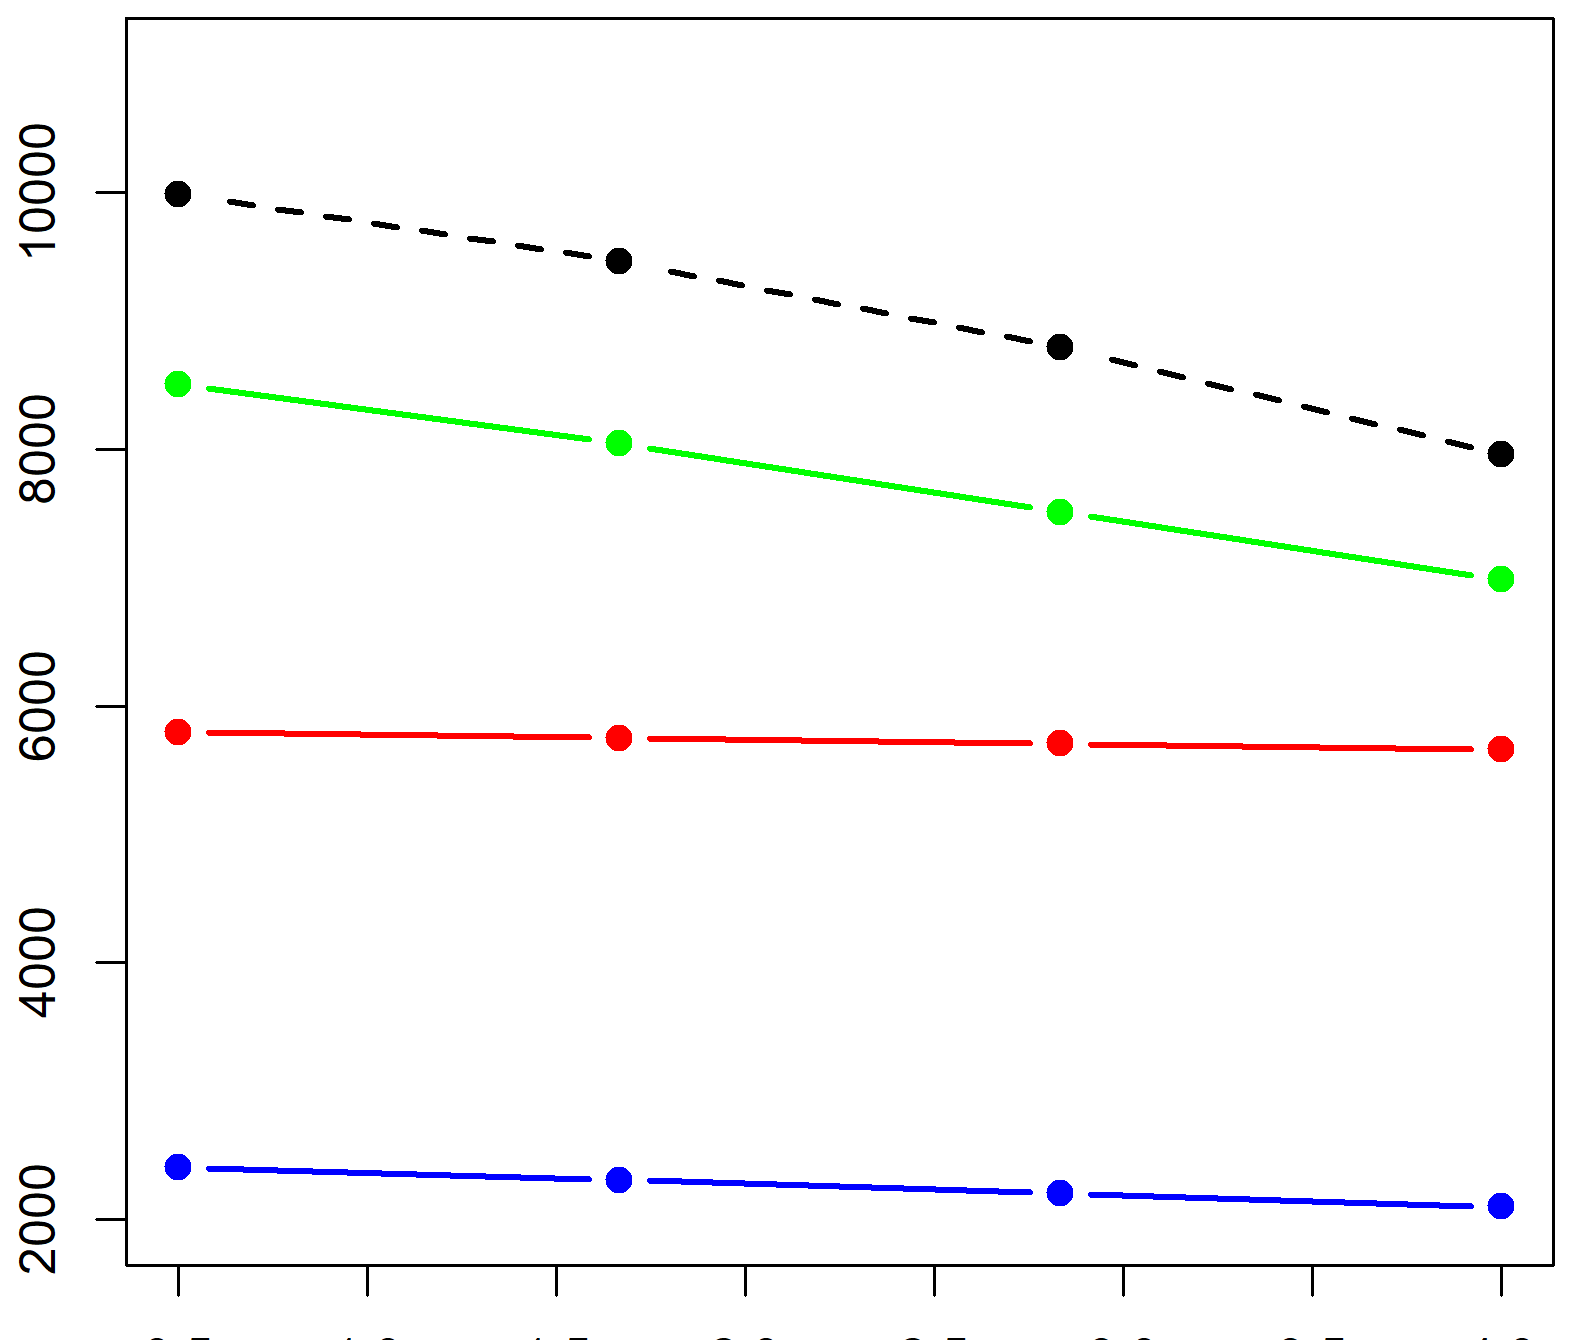
\includegraphics[scale=.6]{figures/example_figure.png}
    \caption{Example figure.}
    \label{fig:1}
\end{figure}

% ==========================
% ==========================
% ==========================


\end{document}